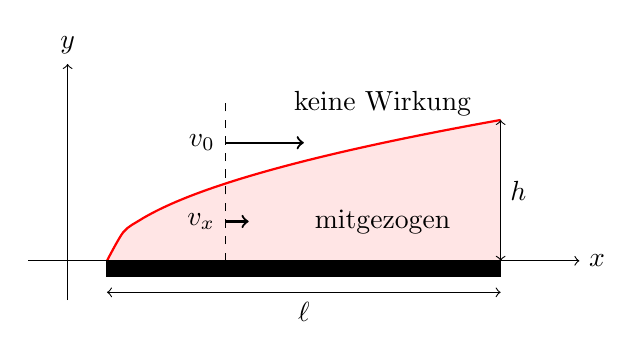
\begin{tikzpicture}
    \pgfmathsetmacro{\k}{.8}
    \pgfmathsetmacro{\lpos}{.5} 
    \pgfmathsetmacro{\l}{5} 
    \pgfmathsetmacro{\vpos}{2}
    
    % block
    \draw[fill] (\lpos,0) rectangle ++(\l,-.2);
    \draw[<->]  (\lpos,-.4) -- node[midway, below] {\(\ell\)} ++(\l,0);
    
    % boundary line and area
    \fill [domain=0:\l, variable=\t, smooth, red!10]
        (\lpos,0)
        -- plot ({\lpos + \t},{\k*sqrt(\t)})
        -- (\lpos + \l,0)
        -- cycle;
    
    \draw[domain=0:\l, variable=\t, smooth, thick, red] (0,0)
        plot ({\lpos + \t},{\k*sqrt(\t)});
    
    % height
    \pgfmathsetmacro{\h}{\k*sqrt(\l)}
    \draw[<->] (\lpos,0) ++(\l,0) -- node[midway, right] {\(h\)} ++(0,\h);
        
    % velocity vectors
    \draw[dashed]    (\vpos,0) -- ++(0,2);
    \draw[->, thick] (\vpos, 1.5) -- node[at start, anchor=east, left] {\(v_0\)} ++(1,0);
    \draw[->, thick] (\vpos, 0.5) -- node[at start, anchor=east, left] {\(v_x\)} ++(.3,0);
    
    % text
    \node at (4,.5) {mitgezogen};
    \node at (4,2) {keine Wirkung};
    
    % axis
    \draw[->] (-.5,0) -- (\l + 1.5,0) node[anchor=west] {\(x\)};
    \draw[->] (0,-.5) -- (0,2.5) node[anchor=south] {\(y\)};
\end{tikzpicture}
